\documentclass[a4paper, oneside]{discothesis}

\usepackage[utf8]{inputenc}
\usepackage[T1]{fontenc}

%%%%%%%%%%%%%%%%%%%%%%%%%%%%%%%%%%%%%%%%%%%%%%%%%%%%%%%%%%%%%%%%%%%%%%%%%%%%%%%%%%%%%%%%%%%%%%%%%
% DOCUMENT METADATA

\thesistype{Semester Thesis} % Master's Thesis, Bachelor's Thesis, Semester Thesis, Group Project
\title{Asynchronous Consensus-Free Transaction Systems}

\author{Shoma Mori}
\email{shmori@student.ethz.ch}

\institute{Distributed Computing Group \\[2pt]
Computer Engineering and Networks Laboratory \\[2pt]
ETH Zürich}

% Optionally, you can put in your own logo here
%\logo{
\includegraphics[width=0.2\columnwidth]{figures/disco_logo_faded}}

\supervisors{Roland Schmid, Jakub Sliwinski\\[2pt] Prof.\ Dr.\ Roger Wattenhofer}

% Optionally, keywords and categories of the work can be shown (on the Abstract page)
%\keywords{Keywords go here.}
%\categories{ACM categories go here.}

\date{\today}

%%%%%%%%%%%%%%%%%%%%%%%%%%%%%%%%%%%%%%%%%%%%%%%%%%%%%%%%%%%%%%%%%%%%%%%%%%%%%%%%%%%%%%%%%%%%%%%%%

\begin{document}

\frontmatter % do not remove this line
\maketitle

\cleardoublepage

\begin{acknowledgements}
    I thank my supervisors Roland Schmid and Jakub Sliwinski for their great support
    during my thesis.
    Special thanks to Prof. Roger Wattenhofer for giving me the opportunity to do this project.
\end{acknowledgements}


\begin{abstract}
In the existing blockchain systems, it is assumed that the consensus problems
should be solved to achieve trust in transactions, while some consensus algorithms cost much.
We introduce Asynchronous Consensus-Free Transaction Systems (ACFTS),
which correctly manages the history of transactions without consensus.
ACFTS dons not need heavy computational power, and the decisions are never overturned
due to its deterministic feature.

We implemented ACFTS as a payment system and evaluated the throughput.
From the results, we found that the parts of creating and verifying signatures
can be bottlenecks.
Furthermore, we can see that it is necessary to improve how to store the transaction data
to get more scalability.
\end{abstract}

\tableofcontents

\mainmatter % do not remove this line

% Start writing here
\chapter{Introduction}

In the existing blockchain systems, it is assumed that the consensus problems
should be solved to achieve trust in transactions.
For instance, Bitcoin~\cite{bitcoin} provides proof-of-work to make consensus
among agents in distributed systems.
Proof-of-work is one of the randomized algorithms using computational power
and spending energy for security of a system, and it requires synchronous communication
among validators.
Proof-of-work needs much computational power to prevent that the history of transactions
is reverted, thus preventing scalability neither.
Furthermore, due to the randomized property, transactions are never finalized,
and can be overturned with decreasing probability.

We introduce Asynchronous Consensus-Free Transaction Systems (ACFTS),
which correctly manages the history of transactions without consensus.
In ACFTS, transactions are approved by the agents called servers,
which dedicate to manage transactions and keep the correctness of the history of transactions.
The servers put their signatures to prove the correctness of transactions.
Importantly, the servers work asynchronously; that is, each server does not communicate
with other servers.
In other words, ACFTS does not need consensus.
Moreover, as ACFTS does work deterministically, once transactions are approved by each server,
the decisions are never overturned.

Gupta \cite{gupta} proposes a financial transfer system which seems to be based
on the similar principles to our system.
In this system, a static set of validators confirms transactions without consensus.

Our system is mainly based on \cite{abc}, which introduces the concept of asynchronous transaction systems without consensus.

We implemented ACFTS as a payment system and evaluated the throughput.
From the results, we found that the parts of creating and verifying signatures
can be bottlenecks.
Furthermore, we can see that it is necessary to improve how to store the transaction data
to get more scalability.

\chapter{Asynchronous Consensus-Free Transaction Systems}

\section{Model}
ACFTS consists of two kinds of agents called servers and clients.
The clients can send cryptocurrency to the other clients or themselves.
In the system, a transaction represents a transfer of cryptocurrency between clients.
Each client holds private and public key pairs
and the public keys are also called addresses, which are used to identify owners of transactions.
The servers verify transactions when they receive them from clients
and record the history of valid transactions in their local storage.

Every client can send messages to all servers and all other clients.
In the same way, every server can send messages to all clients.
However, the servers do not send messages to the other servers.
Messages are delivered asynchronously, that is, messages reach to receivers eventually,
however, there is no guarantee that the messages arrive within finite time.


\section{Protocol}

\subsection{Transaction}
A transaction represents a transfer of cryptocurrency from one client to other clients or itself.
Each transaction consists of one or more inputs and one or more outputs.

An input includes one or more outputs that will be spent.
The output which can be used as an element of inputs is called
a Unspent Transaction Output~(UTXO).
Also, the input has a signature that is generated by a private key
corresponding to the public key (i.e.\ address) of the UTXOs.
In other words, each UTXO can be spent by only the client who knows the private
key which is linked to the public key.
If a client has a private key corresponding to an address of a UTXO,
we say that the client has ownership of the UTXO.

An output includes an address of its owner, amount of cryptocurrency, signatures from servers,
and a hash of outputs of the previous transaction.
In other words, transactions form a directed acyclic graph (DAG).
The sum of the output amount must be the same as one of the input amount.

In the case where a transaction has more than one output, the outputs have \emph{siblings}.
Each output is assigned an index in the siblings.
Normally, outputs can be identified with an address and the previous hash.
However, even if one transaction has multiple outputs that belong to the same addresses
and have the same previous transaction, they are identified by the indexes.

% \TODO{Insert graphs to describe the structure of transactions.}

\subsubsection{Genesis}
All outputs are created from any inputs, but only the genesis is different.
The genesis is an initial output and all outputs refer to the genesis as an ancestor.
The genesis is created by the system, its address represents the first owner
and the amount equals to the sum of the cryptocurrency.

\subsection{Server}
A server is a validator who has the role of verifying transactions from clients.
Every server records all transactions they verified in their memories.
When a server receives a transaction, at first, the server checks
whether the outputs of the received transaction have been used in the past.
If even one of them has been used, the transaction is regarded to be invalid
and the server sends an error to the client.
Next, if the transaction is valid, the server verifies a client's signature
to confirm the ownership.
Then, the server verifies signatures of servers which are also contained in the inputs.
We assume that each server knows the public keys of all the other servers.
Importantly, the number of valid signatures must be more than two-thirds of all servers
to use the UTXOs to prevent from \emph{double-spending}
(the details will be described in \ref{sub:double-spending}).
A UTXO that has signatures from more than two-thirds of all servers is called a valid UTXO.
Finally, the server checks if the sum of the output amount is the same as one of
the input amount.
When the server completes the verification process without any errors,
it approves the transaction by making an own signature from the hash of the outputs
using a private key of the server and attaches it to the response to the client.
The number of signatures of one server for each transaction is only one,
which means the signature is created from the entire outputs, not from each output.
This reduces the number of necessary signatures and saves the cost as a result.
Finally, the server adds the outputs into their storage
and updates the status of the inputs to record that they cannot be used anymore.


\subsection{Client}
Clients can create new transactions.
They send requests for getting signatures from servers to make the transaction valid.
The client manages not only their own outputs but also their sibling outputs
because servers make a signature from the entire outputs in each transaction.
Therefore, the client needs to send the UTXOs with the siblings
in order to make it possible for servers to verify them.
The client attaches a signature to claim the ownership of the UTXOs when sending the request.

Consider a transfer of cryptocurrency from client $c_1$ to client $c_2$.
First, $c_1$ sends a request for the transaction to all servers and waits for the responses.
When $c_1$ gets signatures from more than two-thirds of all servers,
the transaction is regarded to be \emph{approved}.
In order to show the use of the UTXOs and make it possible for $c_2$ to use the new outputs,
$c_1$ sends $c_2$ the outputs with signatures of the servers.
$c_2$ can confirm the correctness of the transaction by verifying the signatures.

\subsection{The flow of a payment}
The following is a flow of creating a transaction
that represents a transfer of the cryptocurrency from client $c_1$ to $c_2$.

\begin{enumerate}
    \item $c_1$ finds valid UTXOs which $c_1$ owns in their local storage.
    \item $c_1$ creates a request for a transaction whose output address represents $c_2$ using the UTXOs and signs it with its private key $p_{c_1}$.
    \item $c_1$ sends the request to all servers and waits for the responses.
    \item When servers receive the request, they check that the transaction is sound
        and that the inputs are unspent.
    \item If the transaction is valid,
        servers create their signatures and send them back as responses.
    \item When $c_1$ gets signatures from more than two-thirds of all servers,
        $c_1$ sends the output of the new transaction to $c_2$.
    \item $c_2$ can confirm that the number of valid signatures is more than two-thirds
        of the number of all servers to check if the transaction is approved.
\end{enumerate}


\subsection{Double-spending}
\label{sub:double-spending}
In general transaction systems, using the same outputs more than twice,
so-called \emph{double-spending}, is one of the critical problems.
We call the transactions that use the same UTXO as their inputs conflicting transactions.
In our system, it is impossible to make the conflicting transactions.

Consider a situation where $c_0$ tries to make two conflicting transactions
which are payments to different clients.
If a server receives two conflicting transactions,
it creates a signature for only one transaction whichever comes first.
Therefore, it is impossible for the client to get signatures of both transactions
from the same server.

Let $N$ denote the number of servers.
Note that each server cannot know the status of other servers,
if the transaction itself in a request is valid, they approve the transaction.
Suppose that $c_0$ does not send the request to $f$ servers.
In this situation, the number of the rest servers is $N-f$.
In other words, $N-f$ nodes are required for quorum.
Since $f$ servers of $N-f$ are not trustworthy, $(N-f)-f$ must be greater than $f$,
that is, $N > 3f$.
The smallest $N$ that satisfies this condition is $N=3f+1$.
From this result, we can see that $c_0$ is incapable of making the two conflicting transactions
approved under the condition that it has to get more than two-thirds of servers
(i.e.\ $\geq2f+1$) for each transaction.
Actually, either one or none of the two transactions are approved.

\chapter{Implementation}
In this chapter, we describe the system in terms of implementation.

\section{Structure}
Servers and clients can communicate through the HTTP protocol.
We adopt JSON as the format of messages.
Servers keep waiting for HTTP requests from clients.
Clients send the servers requests when they want to get signatures of new transactions.

Clients can also send messages to the other clients through the HTTP protocol
to notice new UTXOs that are owned by them.
Therefore, clients also keep waiting for HTTP requests as well as servers.

Both servers and clients manage relational databases to record transaction outputs.
The genesis is initially recorded in the client who has it,
and servers approve the transaction whose input is the genesis without any conditions.



\section{Documentation}

\subsection{Address and signature}
ACFTS uses public-key cryptography to show ownership of outputs
and prove that transactions are approved by servers.
The implementation adopts the Elliptic Curve Digital Signature Algorithm (ECDSA)
for key pairs of servers and clients and the verification processes.

A client creates a hash of UTXOs with SHA256 and signs it with a private key
that is generated with ECDSA when creating a new transaction.
A server verifies the signature with the public key of the client
and signs the UTXOs with a private key which is also generated with ECDSA by the server.
The receiver of the transaction can verify the signatures of servers
with the public keys of the servers.

\subsection{Identification of UTXO}
A UTXO has an address, a hash of outputs of the previous transaction and an index in siblings.
We show that UTXOs can be identified with these keys.

Initially, the genesis is the only transaction and there are no identical transactions.
Hash values become the same deterministically if the inputs are identical.
Without collisions of the hash function, if the input is different, the output becomes different.
Therefore, if the contents of the previous transactions are different,
two transactions are distinguished.
Every output becomes different because even if addresses and the hash
of the previous transactions are the same, they have different indexes.
In short, every transaction has a different set of an address,
a hash of outputs of the previous transaction and an index.

However, if the hash values conflict, two outputs can be the same
although it is usually not the problem probabilistically.


\subsection{Change output}
When a client tries to create a request for a transaction,
the client collects UTXOs from their database until the sum of the amounts
becomes larger than or equal to the amount the client wants to send.
If the sum exceeds the necessary amount, the client make \emph{a change output}
to make both ends meet.
In other words, the client makes an output to itself whose amount is equal to
the difference between the input amount and the output amount.


\subsection{Cluster}
In the implementation, multiple client addresses can be managed in one database.
We call this set of addresses a cluster.
When creating transactions in one cluster, it is not necessary to send UTXOs
because they can refer to them through the shared memory.
In some sense, a cluster can be seen as a wallet and transactions in one cluster
represent sorting out UTXOs.
When creating transactions among different clusters, it is required to send the UTXOs to the related clusters.

Clients can use different addresses depending on transactions for protecting privacy.

In the initialization process, each cluster exchanges their addresses and therefore they can decide which cluster they should send UTXOs when creating new transactions.


\chapter{Experiment}
We evaluated the throughput of our system by experiments using some scenarios of transactions.
The system is implemented in Go and was benchmarked in a local environment
using testing package~\cite{testing, flags} in Go.
The benchmarking has been performed on a laptop with Intel Core i5 3.1GHz CPU and 16GB RAM.
We do not assume network delay.

We also profiled the system to find bottlenecks using pprof~\cite{pprof, profiling},
a Go library for profiling and visualization of programs.

\section{Design}
\begin{itemize}
    \item The number of servers: 4
    \item The number of clients (clusters): 2 ($c_0$ and $c_1$)
    \item The number of addresses in each client: 4\\
        ($\{a_0, a_1, a_2, a_3\} \in c_0$ and $\{a_4, a_5, a_6, a_7\} \in c_1$)
    \item The genesis: $amount = 1000000$, $owner = c_0$
\end{itemize}

We executed the following five different scenarios.
Every arrow indicates a transfer of 1 amount of cryptocurrency.
\begin{itemize}
    \item Scenario1: $a_0 \rightarrow a_1$
    \item Scenario2: $a_0 \rightarrow a_1$, $a_1 \rightarrow a_0$
    \item Scenario3: $a_0 \rightarrow a_1$, $a_1 \rightarrow a_0$, $a_2 \rightarrow a_3$, $a_3 \rightarrow a_2$
    \item Scenario4: $random \rightarrow random~(random \in c_0)$
    \item Scenario5: $a_0 \rightarrow a_4$
\end{itemize}
Note that the sender and the receiver are chosen from $c_0$ with equal probability in scenario4.

\section{Results}

\subsection{Processing speed}
"Trials" in the tables means the number of executions of a set of transactions in one scenario.
For example, in scenario1, when the trials is 10, a transaction from $a_0$ to $a_1$
is executed 10 times.
On the other hand, in scenario2, when the trials is 10,
transactions from $a_0$ to $a_1$ and from $a_1$ to $a_0$ are executed 10 times respectively.
Speed is the number of approved transactions per second.
Although there are exemptions, the throughputs go down as increasing the number of transactions.

\begin{table}[t]
    \begin{center}
        \begin{tabular}{c}

            \begin{minipage}{0.5\hsize}
                \begin{center}
                    \caption{Scenario1}
                    \label{tbl:scenario1}
                    \begin{tabular}{|l|c|} \hline
                        trials & speed [tx/s]\\ \hline \hline
                        10 & 5.25 \\
                        100 & 4.27 \\
                        1000 & 4.43 \\ 
                        10000 & 3.49 \\ \hline
                    \end{tabular}
                \end{center}
            \end{minipage}

            \begin{minipage}{0.5\hsize}
                \begin{center}
                    \caption{Scenario2}
                    \label{tbl:scenario2}
                    \begin{tabular}{|l|c|} \hline
                        trials & speed [tx/s]\\ \hline \hline
                        10 &  5.95 \\
                        100 & 5.00 \\
                        1000 & 4.87 \\
                        10000 & 3.52\\ \hline
                    \end{tabular}
                \end{center}
            \end{minipage}

        \end{tabular}
    \end{center}
\end{table}


\begin{table}[t]
    \begin{center}
        \begin{tabular}{c}

            \begin{minipage}{0.33\hsize}
                \begin{center}
                    \caption{Scenario3}
                    \label{tbl:scenario3}
                    \begin{tabular}{|l|c|} \hline
                        trials & speed [tx/s]\\ \hline \hline
                        10 & 5.17 \\
                        100 & 4.58 \\
                        1000 & 4.92 \\
                        10000 & 2.71 \\ \hline
                    \end{tabular}
                \end{center}
            \end{minipage}

            \begin{minipage}{0.33\hsize}
                \begin{center}
                    \caption{Scenario4}
                    \label{tbl:scenario4}
                    \begin{tabular}{|l|c|} \hline
                        trials & speed [tx/s]\\ \hline \hline
                        10 & 5.33 \\
                        100 & 5.52 \\
                        1000 & 5.44 \\
                        10000 & 4.54 \\ \hline
                    \end{tabular}
                \end{center}
            \end{minipage}

            \begin{minipage}{0.33\hsize}
                \begin{center}
                    \caption{Scenario5}
                    \label{tbl:scenario5}
                    \begin{tabular}{|l|c|} \hline
                        trials & speed [tx/s]\\ \hline \hline
                        10 &  5.38 \\
                        100 & 5.23 \\
                        1000 & 4.29 \\
                        10000 & 3.14 \\ \hline
                    \end{tabular}
                \end{center}
            \end{minipage}

        \end{tabular}
    \end{center}
\end{table}


\subsection{Bottlenecks}
We employed flame graphs to find bottlenecks of the system.

\subsubsection{Flame graph}
Flame graphs~\cite{flame} are a visualization that allows identifying
the most frequent code-paths.
The y-axis shows the stack depth, ordered from root at the top to leaf at the bottom.
The x-axis spans the stack trace collection.
The width of each function box shows the frequency at which that function was present
in the stack traces, or part of a stack trace ancestry.
In the flame graphs, bottleneck functions should be shown as wide width boxes.

We profiled a client program and a server program when executing scenario1 (trials = 10000).
In order to investigate the difference of the CPU status depending on timing,
we analyzed the programs during the first 60 seconds and the last 60 seconds of the execution.

Figure~\ref{fig:fg-server-b} shows the analysis result of a server during the first 60 sec and
Figure~\ref{fig:fg-server-e} shows the one during the last 60 seconds.
Figure~\ref{fig:fg-client-b} shows the analysis result of a client during the first 60 sec and
Figure~\ref{fig:fg-client-e} shows the one during the last 60 seconds.

\begin{figure}[p]
    \begin{center}
        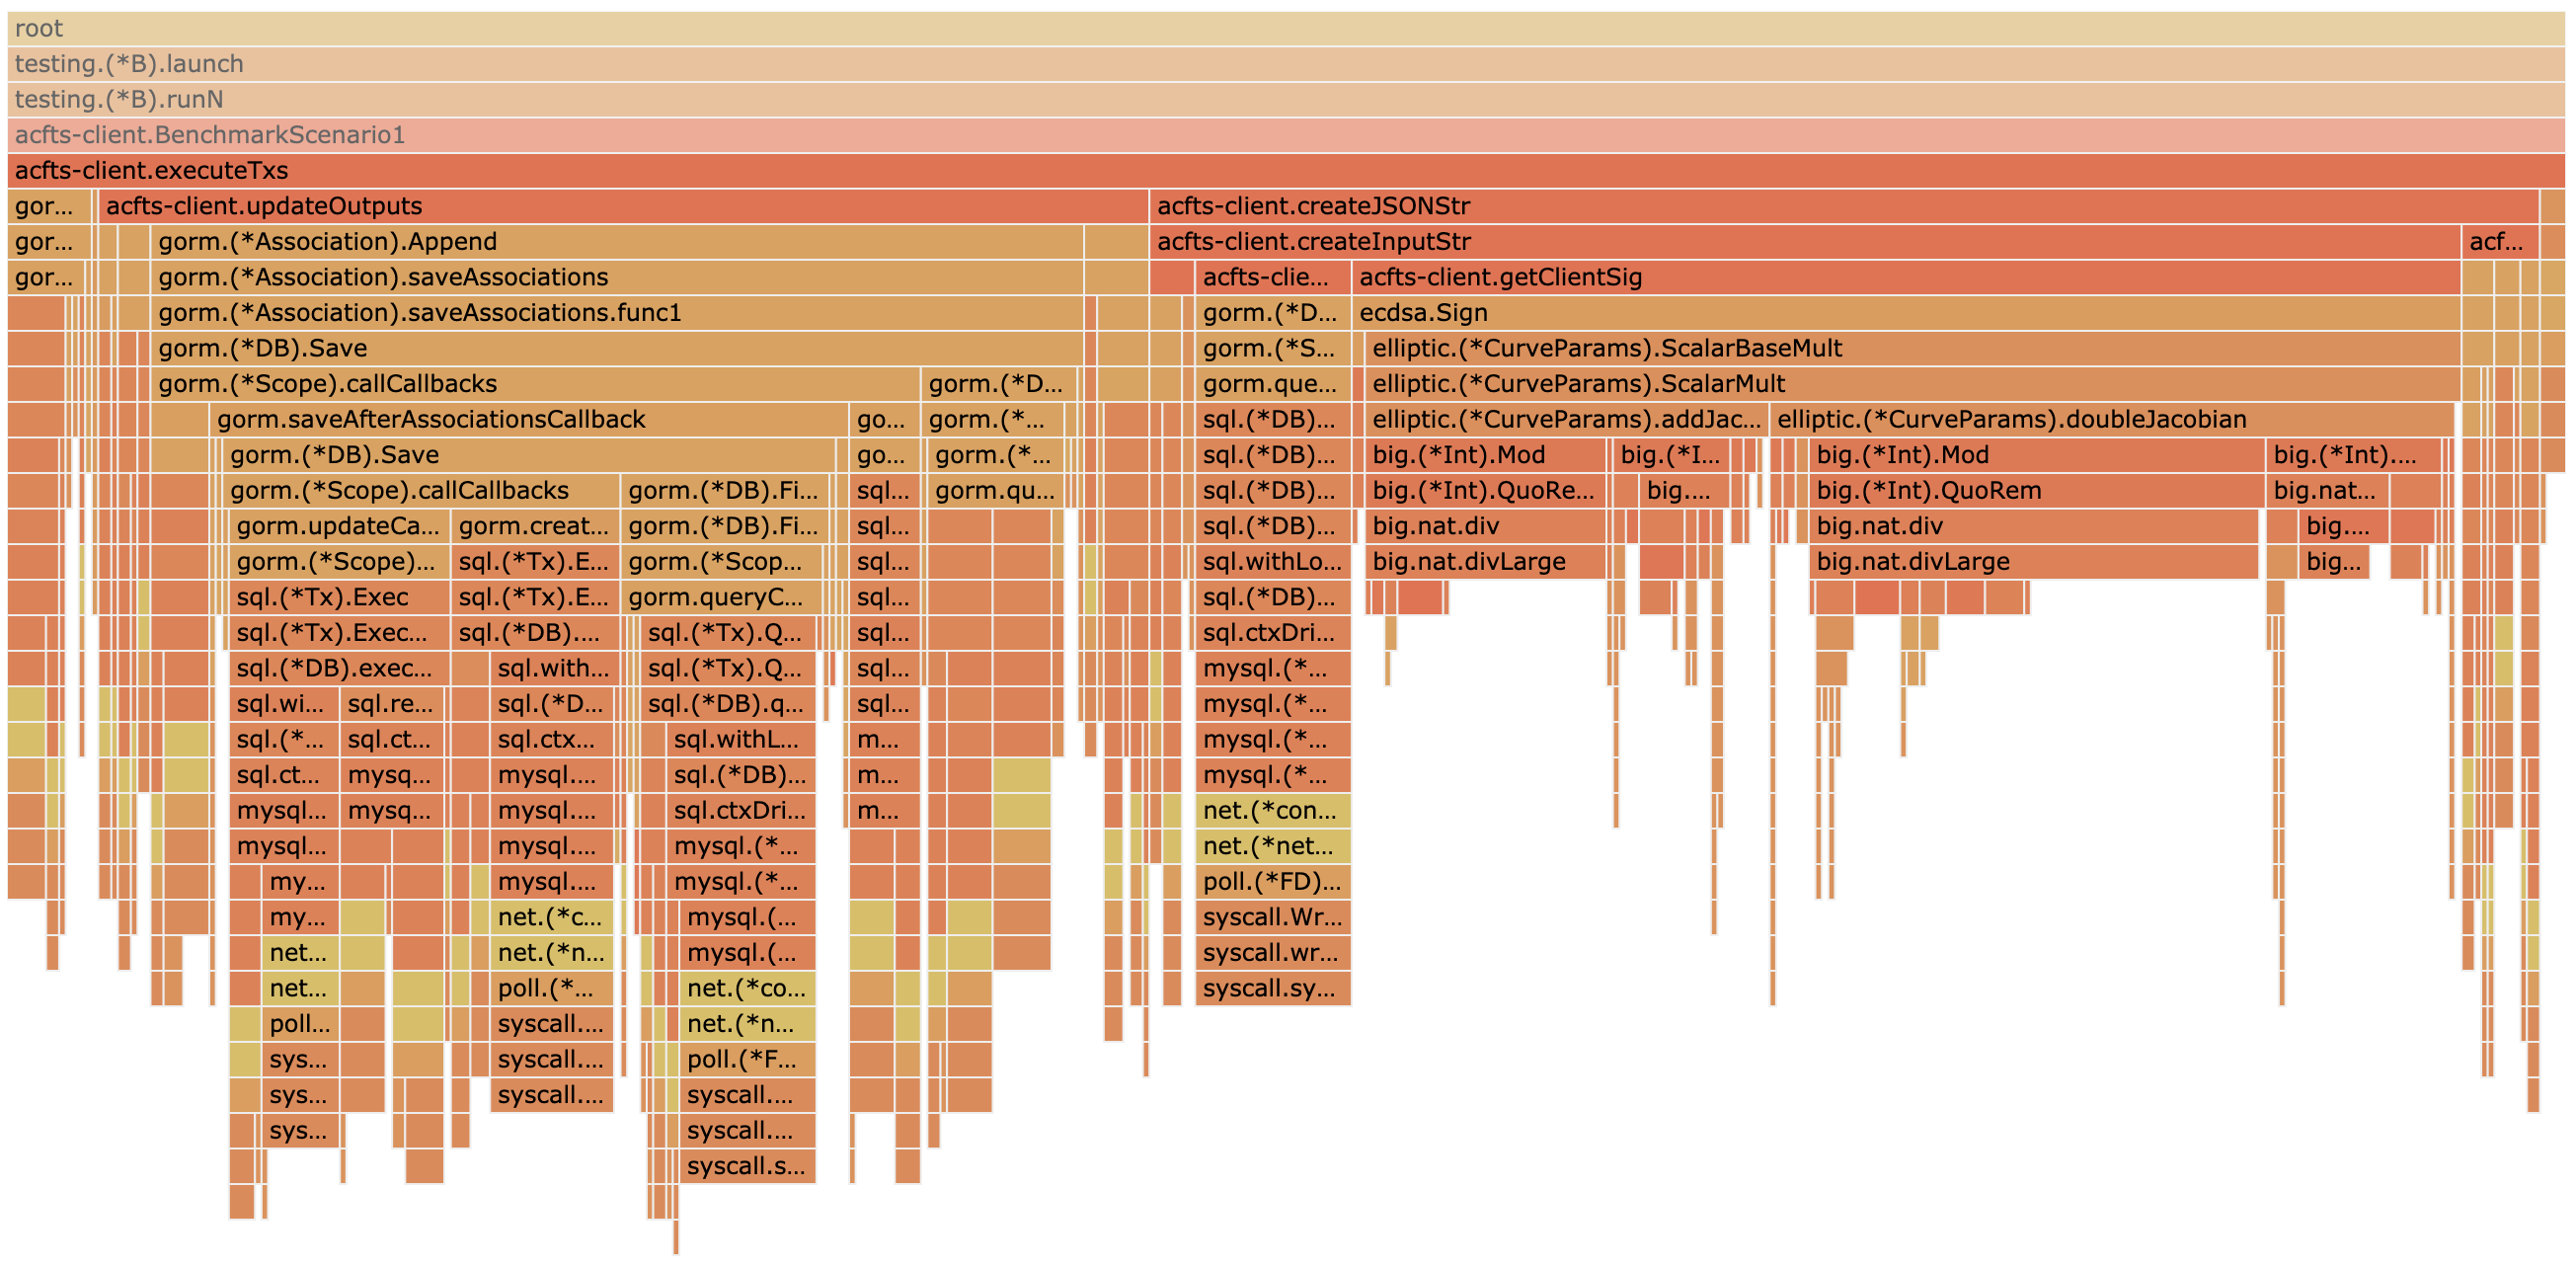
\includegraphics[width=\columnwidth]{figures/flame_graph_client_begining}
        \caption{The flame graph in a client during the first 60 seconds of the execution}
        \label{fig:fg-client-b}
    \end{center}
\end{figure}

\begin{figure}[p]
    \begin{center}
        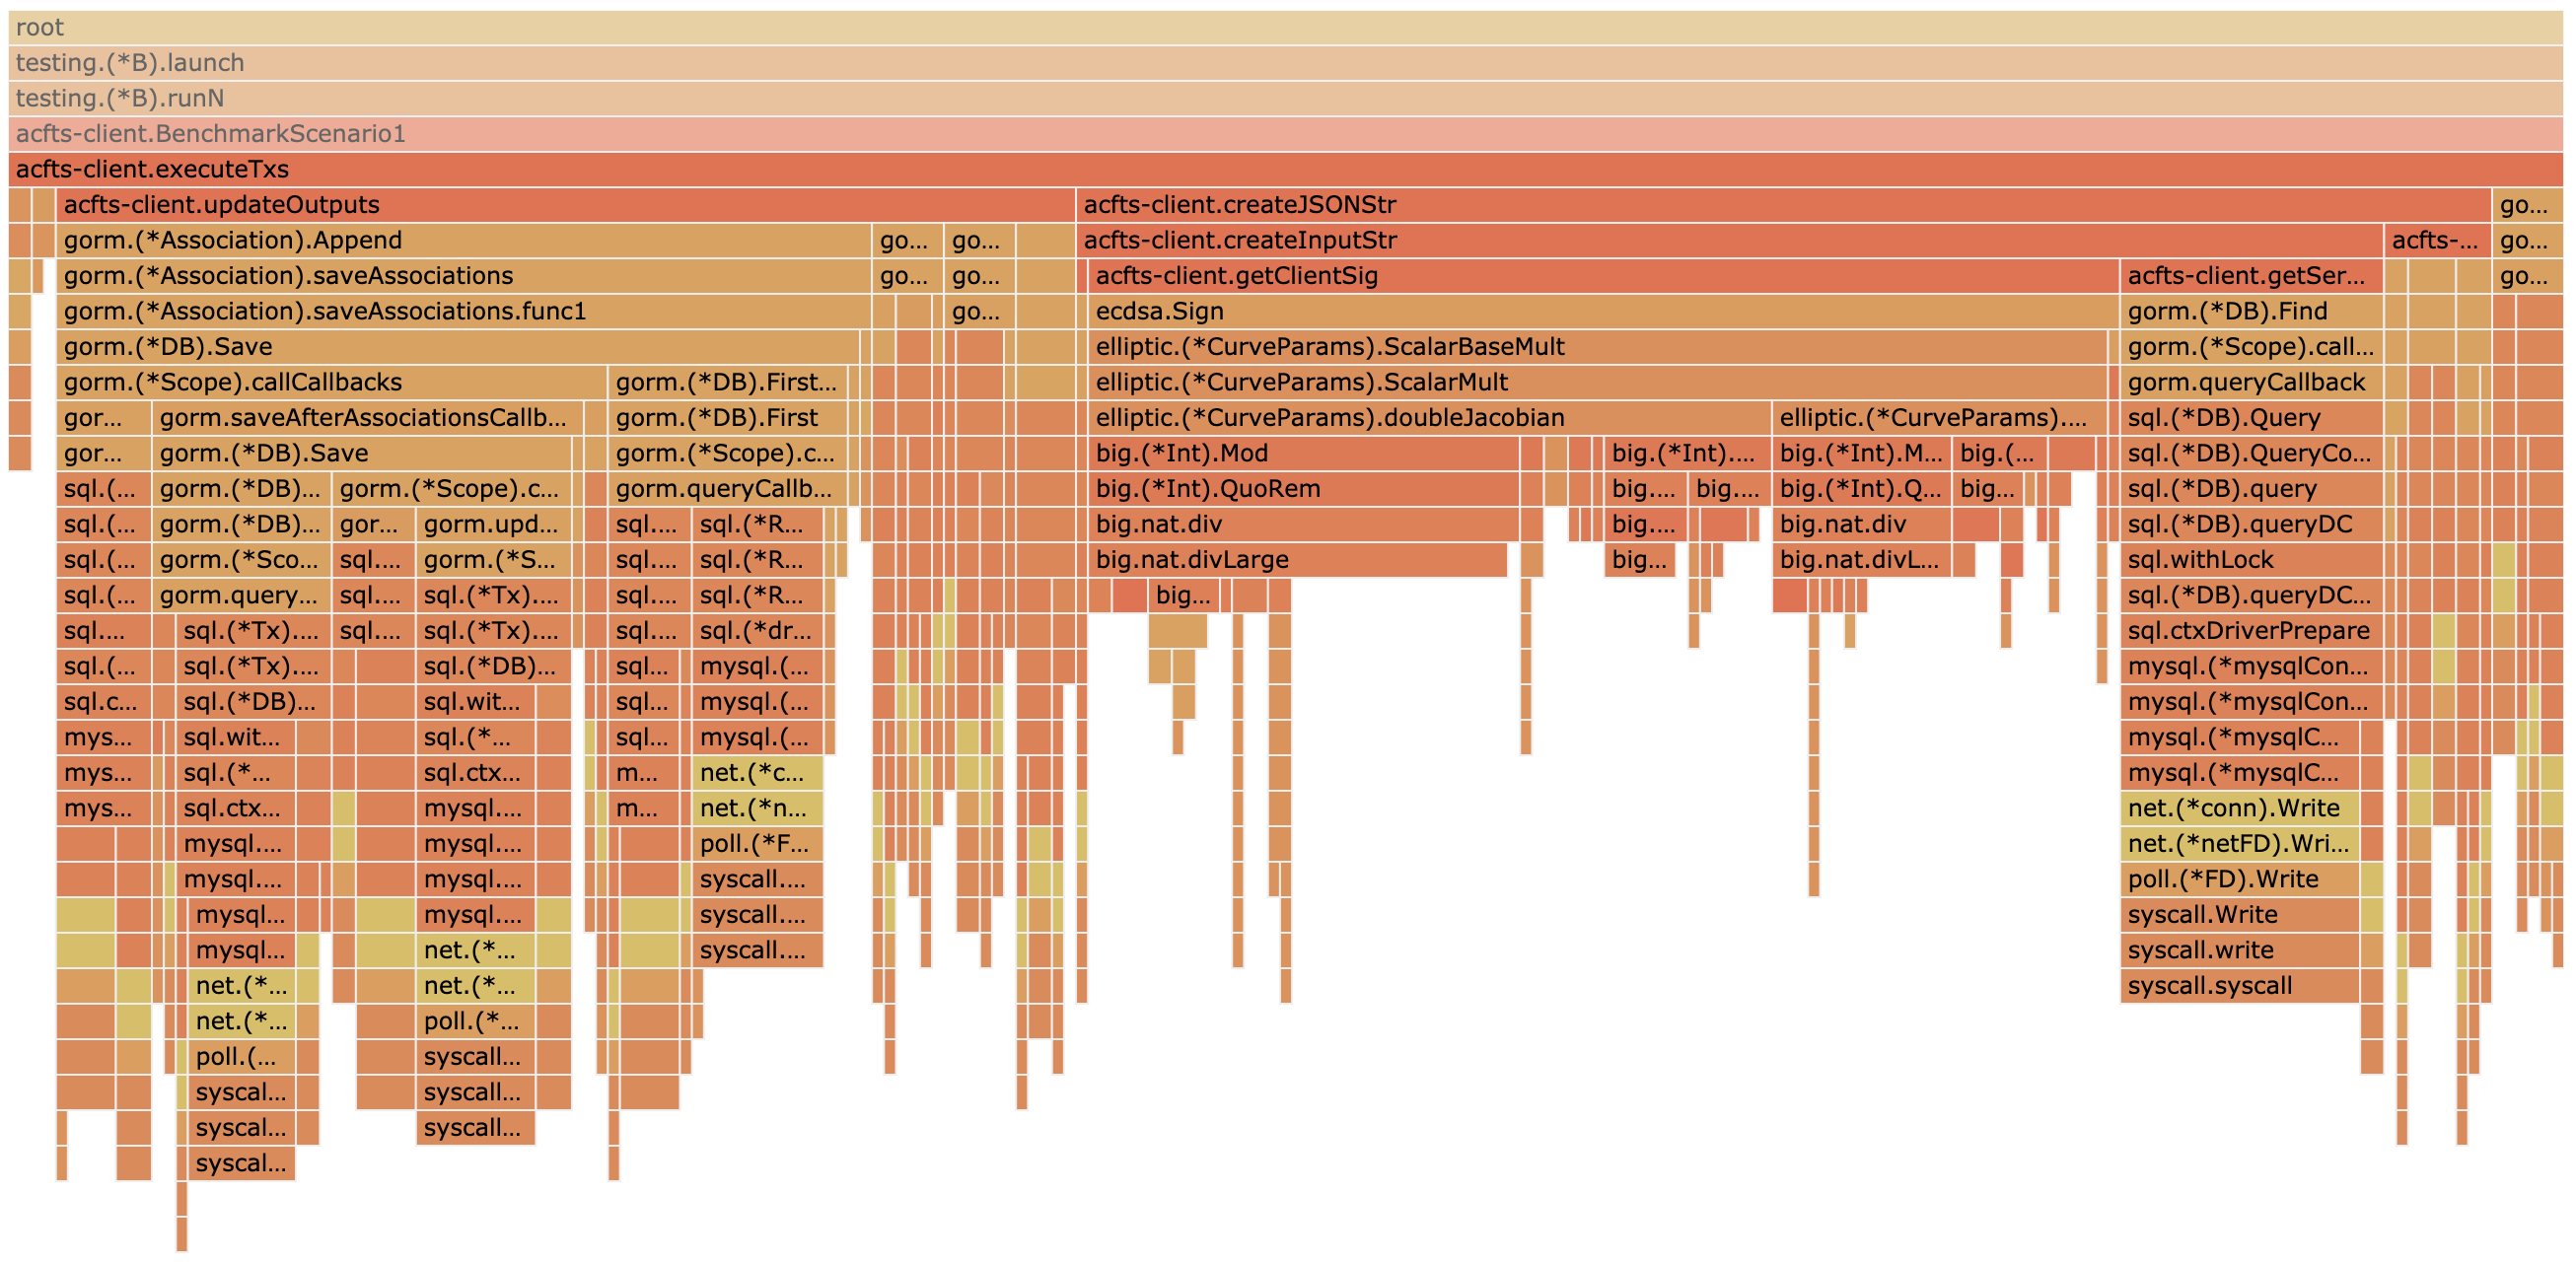
\includegraphics[width=\columnwidth]{figures/flame_graph_client_ending}
        \caption{The flame graph in a client during the last 60 seconds of the execution}
        \label{fig:fg-client-e}
    \end{center}
\end{figure}


\begin{figure}[p]
    \begin{center}
        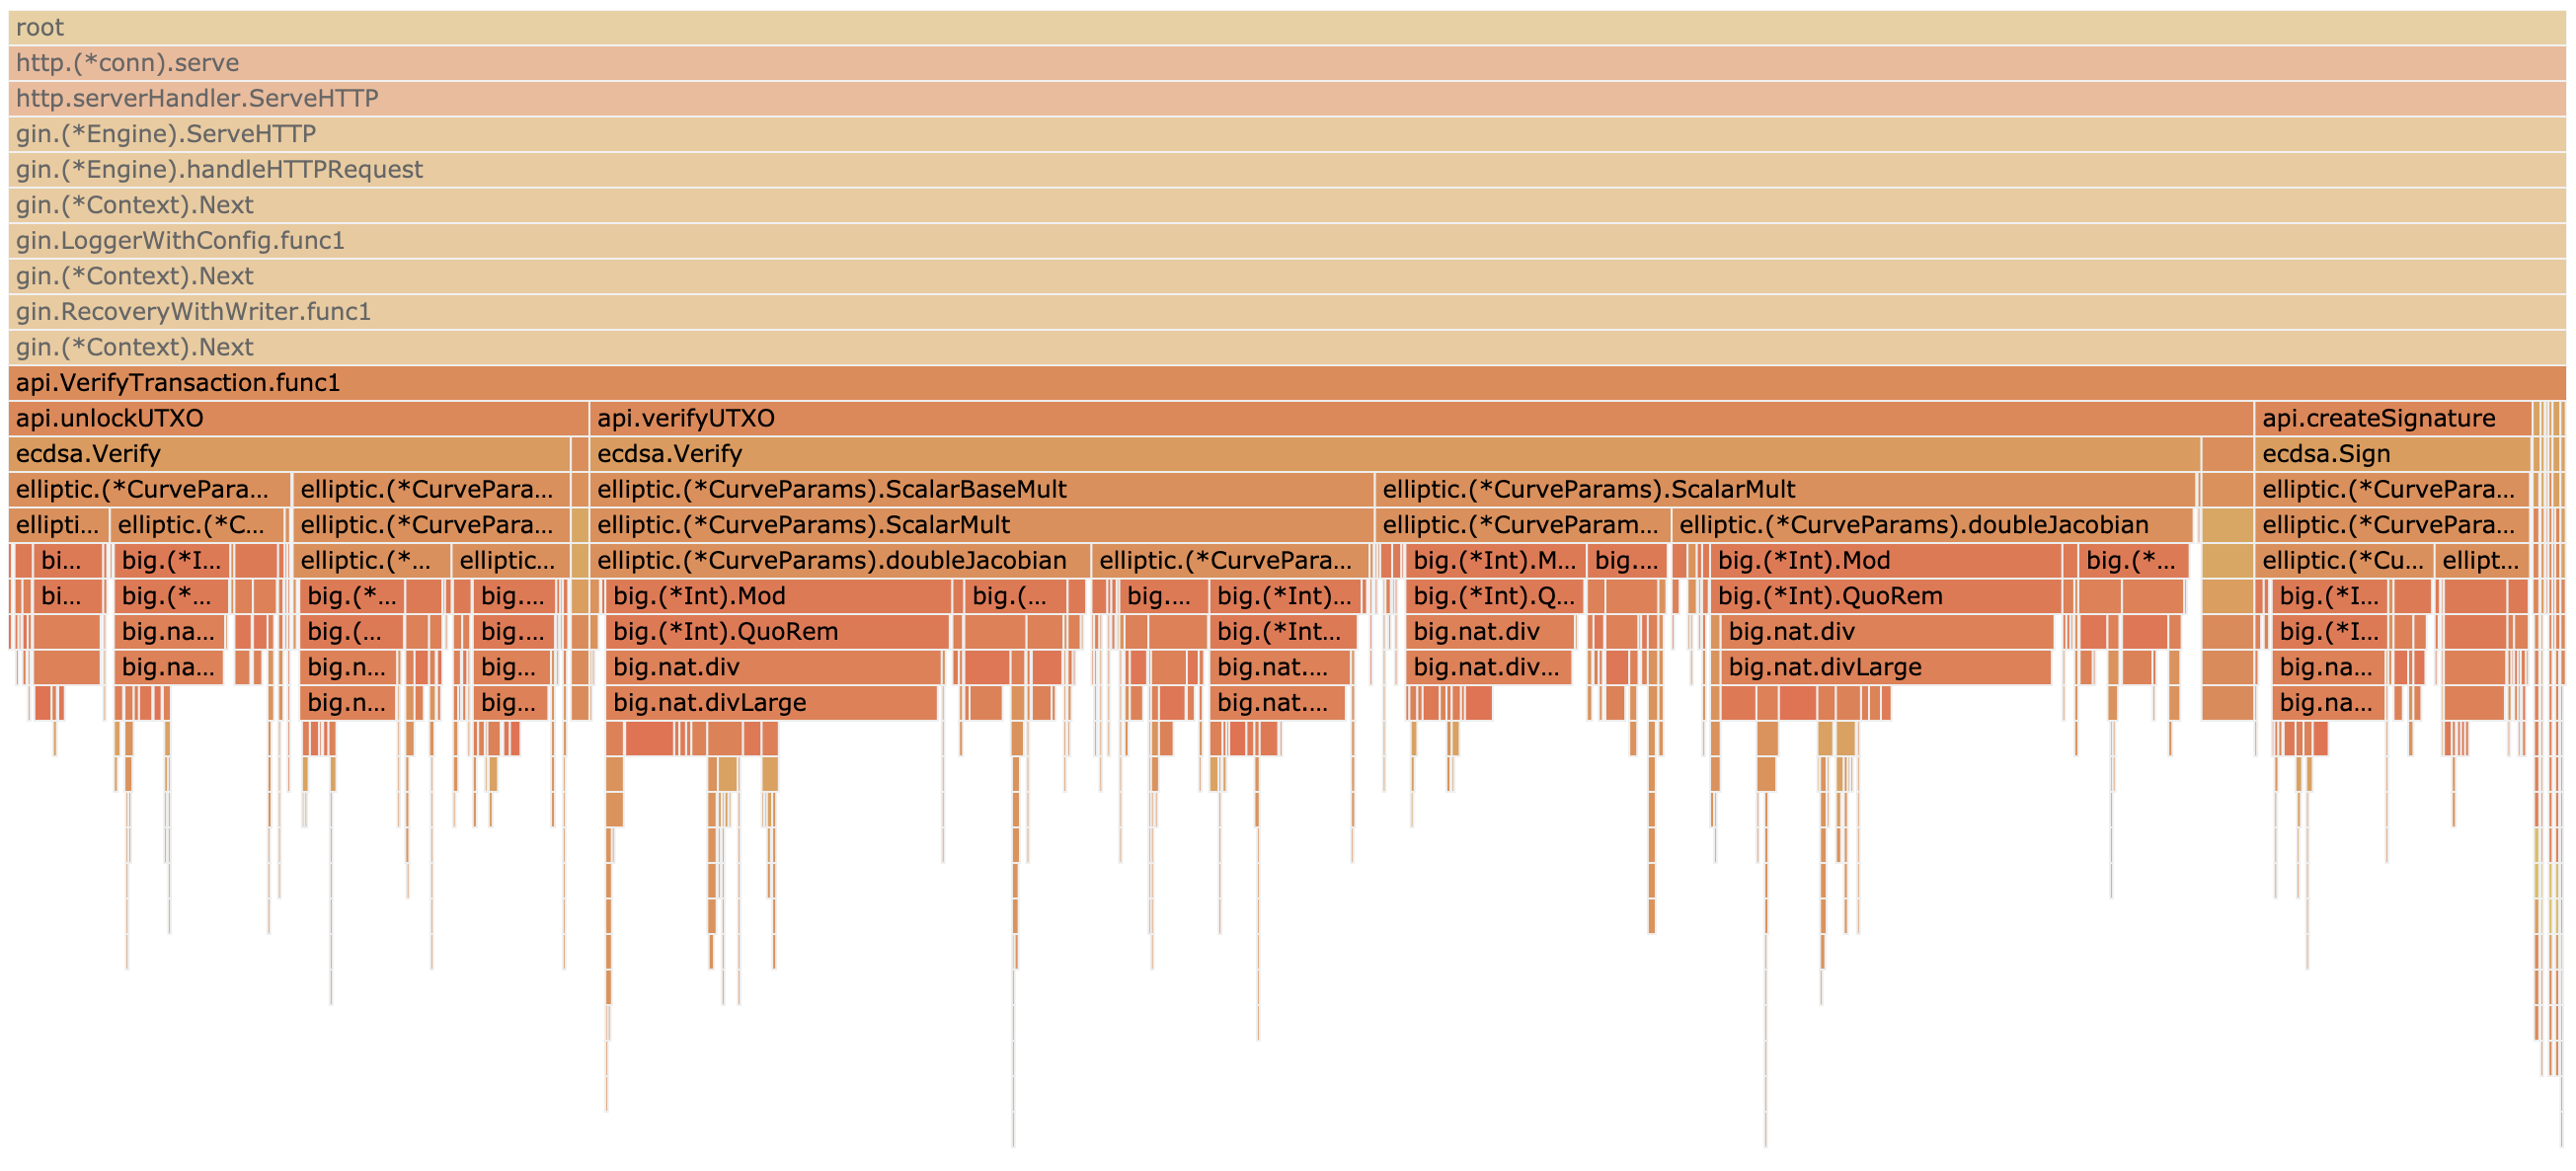
\includegraphics[width=\columnwidth]{figures/flame_graph_server_begining}
        \caption{The flame graph in a server during the first 60 seconds of the execution}
        \label{fig:fg-server-b}
    \end{center}
\end{figure}

\begin{figure}[p]
    \begin{center}
        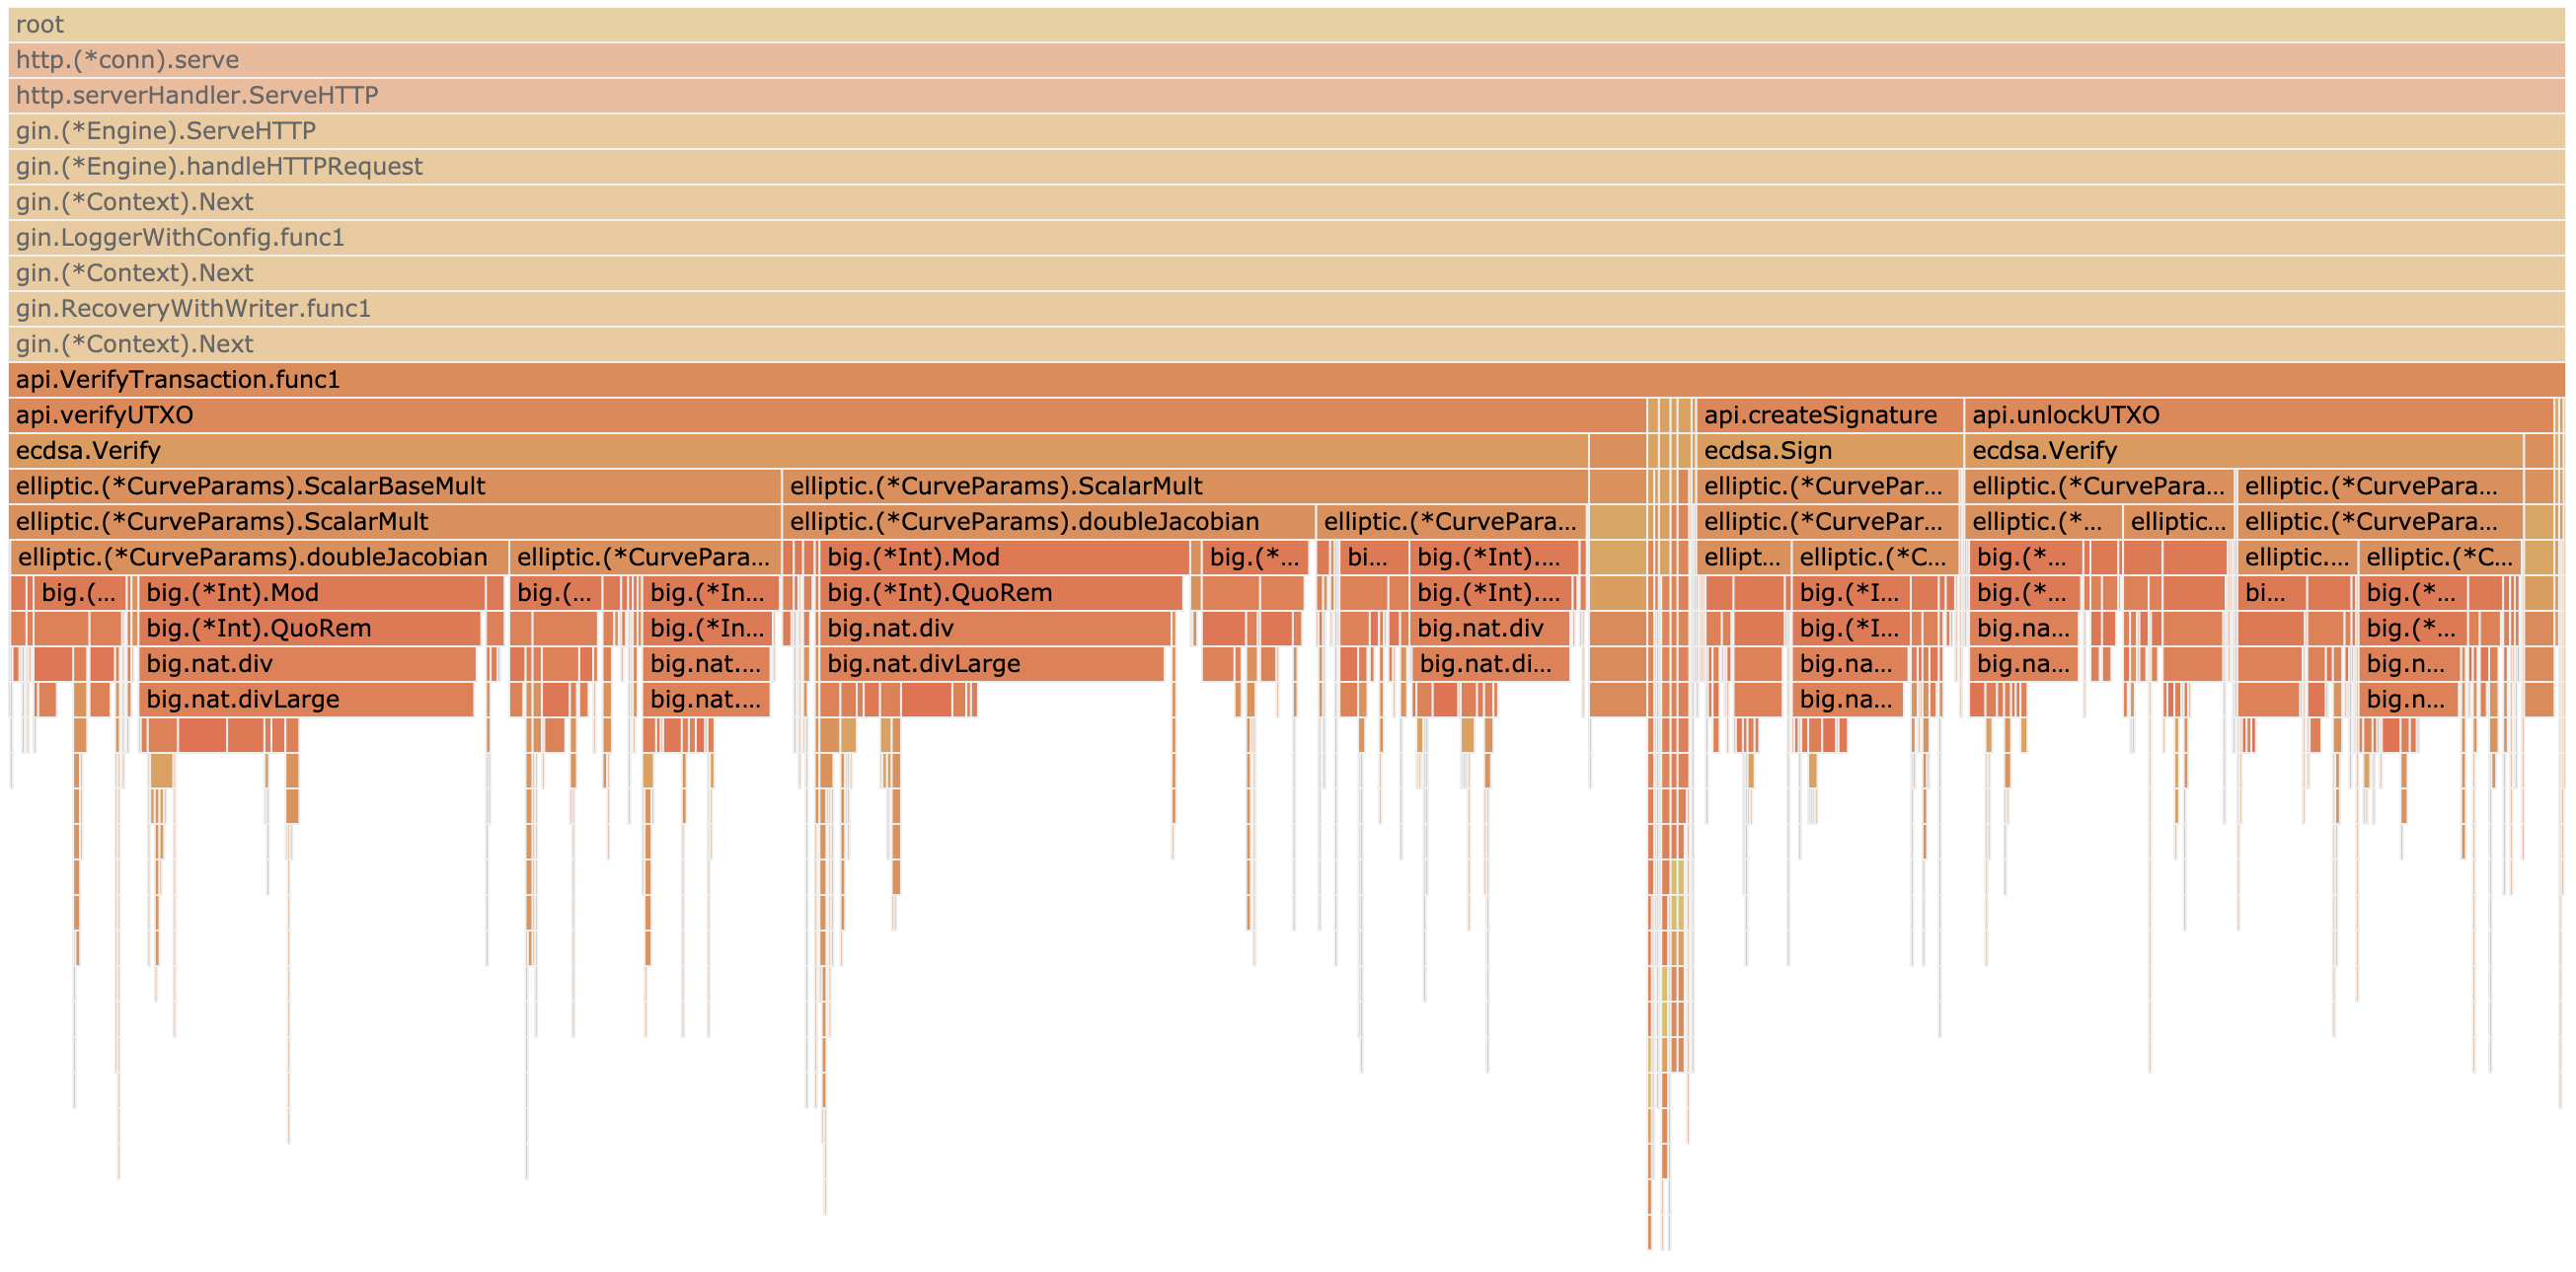
\includegraphics[width=\columnwidth]{figures/flame_graph_server_ending}
        \caption{The flame graph in a server during the last 60 seconds of the execution}
        \label{fig:fg-server-e}
    \end{center}
\end{figure}

In a client program, acfts-client.executeTxs is a function that creates requests,
sends them to all servers, waits for responses and updates the output table in the database.
From Figure~\ref{fig:fg-client-b} and \ref{fig:fg-client-e}, we can see
that acfts-client.createJSONStr and acfts-client.updateOutputs account for
the most of CPU when acfts-executeTxs is on the stack.
acfts-client.createJSONStr is a function that makes JSON string for a request.
The resource of acfts-client.createJSONStr is used mainly by acfts-client.findUTXOs,
acfts-client.getClientSig, and acfts-client.getServerSigs.
acfts-client.findUTXO is a function that finds valid UTXOs from the database.
acfts-client.getClientSig is a function that creates a signature of the client
to show the ownership of the UTXOs.
This calls ecdsa.Sign which is one of the library functions that makes a signature.
acfts-client.getServerSigs is a function that selects the server's signatures
of each UTXO from the database.
acfts-client.updateOutputs is called when a client receives responses from servers.
It creates new outputs and adds signatures from servers.
gorm.(*Association).Append is a function of GORM~\cite{gorm},
a Object-relational mapping (ORM) library in Go,
which is called when adding the signatures to the database.

Table~\ref{tbl:bn-client} shows the ratios of CPU use of each function
to acfts-client.executeTxs in the two periods.
It is found that the ratios of acfts-client.getServerSig and acfts-client.findUTXOs increased
from the first 60 sec to the last 60 sec.
These two functions search specific records from the tables of signatures
and outputs respectively.
\begin{table}[t]
    \begin{center}
        \caption{The ratios of main functions to executeTxs}
        \label{tbl:bn-client}
        \begin{tabular}{|c|c|c|} \hline
            name & first 60s [\%] & last 60s [\%] \\ \hline \hline
            getClientSig & 43.4 & 40.4 \\
            getServerSigs & 6.13 & 10.3 \\
            findUTXOs & 3.06 & 4.23 \\ \hline
            % & 52.59 & 54.93 \\ \hline
            updateOutputs & 41.0 & 39.9 \\ \hline
        \end{tabular}
    \end{center}
\end{table}
\begin{table}[t]
    \begin{center}
        \caption{The ratios of main functions to VerifyTransaction}
        \label{tbl:bn-server}
        \begin{tabular}{|c|c|c|} \hline
            name & first 60s [\%] & last 60s [\%] \\ \hline \hline
            verifyUTXO & 65.1 & 64.1 \\
            unlockUTXO & 22.7 & 23.1 \\
            createSignature & 10.9 & 10.5 \\ \hline
        \end{tabular}
    \end{center}
\end{table}

In a server program, api.VerifyTransaction is called at first
when receiving requests from clients.
As we can see Figure~\ref{fig:fg-server-b} and \ref{fig:fg-server-e}, it is found
that api.verifyUTXO, api.unlockUTXO and api.createSignature are the dominant functions.
If we trace the stacks, we can see that ecdsa.Verify and ecdsa.Sign are called in each function.
ecdsa is a cryptographic library of the Elliptic Curve Digital Signature Algorithm~\cite{ecdsa}
in Go.
In api.verifyUTXO, a server verifies server's signatures of the receiving UTXOs in the inputs.
In api.unlockUTXO, a server verifies client's signatures of each UTXO which the client attached.
In api.createSignature, a server issues a signature to prove the correctness of the transaction.

Table~\ref{tbl:bn-server} shows the ratios of CPU use of each function to api.VerifyTransaction.
There are no significant differences between the first 60 sec and the last 60 sec,
meaning that the efficiency of the server does not change
depending on the number of transactions.

\section{Discussion}

\subsection{Client database bottleneck}
From the results of the benchmark, we found that throughputs go down
as increasing the number of transactions.
According to the results of the profiling (Table~\ref{tbl:bn-client}, \ref{tbl:bn-server}),
it is thought that the cause derives from acfts-client.getServerSigs and acfts-client.findUTXOs.
It is because the ratios of CPU use of these functions go up
while the others do not change so much as the number of transactions increases.
These two functions get records of signatures and outputs from the tables in the database.
The more the number of transactions increases,
the more the number of records that the program has to look up.
As a result, the processing speed goes down.

Although we have set indexes on the tables of outputs and signatures
to search records effectively~\cite{mysql, multiple},
the costs still rise as increasing the number of records.
It is required to remove the bottlenecks to get more scalability.

As for the signatures, it will be enough to save them in a hash table whose inputs are
an address, the previous hash and an index of a UTXO and outputs are the signatures.
On the other hand, regarding the outputs, acfts-client.findUTXOs has to search UTXOs
which are owned by the client until the sum of the amounts becomes larger than or equal to
the necessary amount.
If the outputs are saved in a hash table whose input is an address and outputs are
an array of UTXOs, it is required to look up UTXOs linearly after all.
It also costs much when the number of transactions is large.

One of the possible improvements is that periodically, making transactions
within each cluster that put together some outputs which are owned by the same addresses.
The reason why acfts-client.findUTXOs can be a bottleneck is that that has to
look up a large number of outputs many times.
Therefore, if the number of outputs to be looked up decreases, the cost should decrease too.


\subsection{Transaction between different clusters}
One of the ways to improve the throughput of transactions among clusters is not to wait
for the responses from the receiver cluster.
Actually, in the real use of this system such as payment in a cafe,
it is enough for a payer to send signatures of servers in some way
or just show something (e.g.\ QR code) which has the information to a payee.
Then, the payee does not need to respond in some digital way.


\subsection{Waiting for signatures from servers}
Currently, clients wait for responses from all servers
after they sent requests for new transactions.
However, it is enough if they have more than two-thirds of all signatures
to show the validity of the new transactions.
Suppose that a client sends a valid transaction and all servers will send signatures back.
If the client does not wait after getting more than two-thirds of all signatures,
the processing speed will 1.5 times faster.


\subsection{Algorithm for cryptographic processes}
The most of spending time in a server is attributed to cryptographic processes
such as creating signatures and verification of the signatures.
There are no specific reasons why we must adopt ECDSA as the algorithm
for the cryptographic processes.
We can take into account other cryptographic algorithms for our system.
Go provides some libraries for other algorithms
such as RSA~\cite{rsa} and the Digital Signature Algorithm~(DSA)~\cite{dsa}.


\subsection{Changes of servers}
Now, the number of servers and their addresses are fixed.
However, if the servers are fixed permanently, they will be a vulnerability
when some of them stop or break.
To avoid that situation, the system should adapt to the replacement of servers.
Now, there are no ways for servers to let clients know the replacement of themselves.


\subsection{Run in a real environment}
The experiments do not consider network delay.
However, that can be a critical issue when measuring the throughput in a real environment.
It is thought that measurement using a real environment such as a public cloud service is needed.


\chapter{Conclusion}
In this thesis, we implemented ACFTS, asynchronous consensus-free transaction systems.
ACFTS provides the functionality that approves only correct transactions without consensus.
The servers who verify transaction work without communication among them,
and therefore they do not need synchronization.

On the other hand, the results of the experiments have shown that
making and verifying signatures cost time.
Moreover, the more the number of approved transactions increases,
the more creating new transactions takes.
We can see that it is required to improve how to store transactions to get scalability.
As future work, we should consider changing how to store outputs
and making the system adapt to the replacement of servers.

% This displays the bibliography for all cited external documents. All references have to be defined in the file references.bib and can then be cited from within this document.
\bibliographystyle{IEEEtran}
\bibliography{references}

% This creates an appendix chapter, comment if not needed.
% \appendix
% \chapter{First Appendix Chapter Title}

\end{document}
